
\section{Introduction to PIRS}
\subsection{What it is}
% Definition with explanation
\begin{frame}\frametitle{What is PIRS}

    \begin{block}{PIRS: Python Interfaces for Reactor Simulations}

        A package for \uline{Python} programming language, to facilitate
        \uline{interaction} with reactor calculation codes.
    \end{block}

    \begin{columns}
        \column{0.45\textwidth}

        \pause
        \begin{block}{Python}
        \begin{itemize}

            \item www.python.org

            \item Free 

            \item Interpreted: cross-platform but slow

            \item Big community: lot of ready-to-use solutions


        \end{itemize}
        \end{block}

        \column{0.45\textwidth}

        \pause
        \begin{block}{Interaction with code}
        \begin{itemize}
            
            \item Model description

            \item Generation of Input file(s)

            \item Job submission

            \item Reading of calculation results

        \end{itemize}
        \end{block}
    \end{columns}
\end{frame}

% History: why Python, task behind: coupling MCNP and SCF, build principles (light-weight, general tool, modular)
\begin{frame}\frametitle{Background}
    \begin{block}{Prerequisites}
    \begin{itemize}
        \item Author's Experience with Python and MCNP 
        \item HPMC project: goal to couple Monte-Carlo with TH for PWR-like geometries from pin to reactor core
        \item Previous coupling schemes -- mix of programming languages (from shell to fortran), higly specific to geometry
    \end{itemize}
    \end{block}

    \begin{block}{Idea}
    \begin{itemize}
        \item Light-weight: e.g. to deploy on cluster's local account
        \item General tool: geometry-independent, not only for coupled calculations
        \item Everything should be specified in terms of a programming language
    \end{itemize}
    \end{block}
\end{frame}

\begin{frame}\frametitle{PIRS concept}
    % when implementing coupled calcs from scratch, one needs to define things that can be put into several types:
    %    * data common to all codes, i.e. geometry description of calculational model, meshes to represent dependent variables
    %    * code-specific data like material composition or T/H properties
    %    * organization of data flow

    \begin{itemize}
        \item Geometry definition: should be reusable in all codes, defined in terms, independent on any particular code.

        \item Convenien way to handle distribution of dependent variables (heat deposition, temperature and material density axial distributions)

        \item Interface consists of two parts:
            \begin{itemize}
                \item Low-level interface: "knows" syntax of input file(s), can read output files, can start code and wait until it completes
                \item High-level interface: converts code-independent geometry together with additionally specified code-specific data to low-level interfaces, and puts results of
                      calculations back to code-independent geometry.
            \end{itemize}
    \end{itemize}
\end{frame}


\subsection{Concept}
% Interface concept: show the scheme, explain data flow, explain what user and developers use.
\begin{frame}[fragile]
    \frametitle{PIRS concept scheme}
    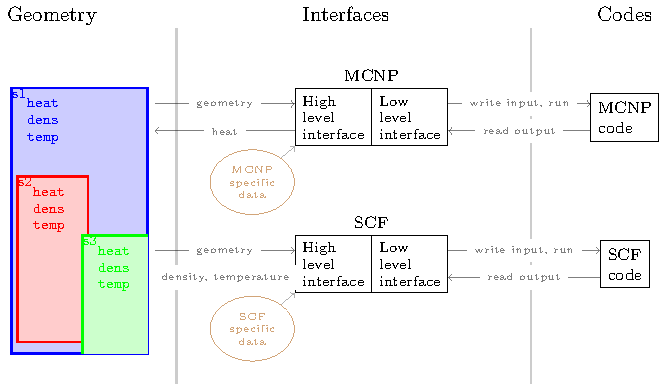
\includegraphics[width=\textwidth]{scheme_wrapper.pdf}
\end{frame}



\subsection{Content}
% Package content: list of subpackages, only general overview
\begin{frame}[fragile]
    \frametitle{PIRS classes and functions}

    \begin{block}{Geometry construction}
    \begin{columns}
        \column{0.6\textwidth}
        \begin{pythoncode}
            from pirs.solids import Cylinder, Box
            from pirs.solids import zmesh
        \end{pythoncode}
        \column{0.4\textwidth}{\scriptsize

        Classes to represent solids -- basic elements to describe geometry and axial meshes for dependent variables.

        }
    \end{columns}
    \end{block}

    \begin{block}{High-level interfaces}
        \begin{pythoncode}
            from pirs import McnpInterface
            from pirs import ScfInterface
        \end{pythoncode}
    \end{block}
\end{frame}


\begin{frame}[fragile]
    \frametitle{PIRS classes and functions}

    \begin{block}{Low-level interface to MCNP}
    \begin{columns}
        \column{0.8\textwidth}
        \begin{pythoncode}
        from pirs.mcnp import Material, MaterialCollection
        from pirs.mcnp import MeshTally, TallyCollection
        from pirs.mcnp import Xsdir
        from pirs.mcnp import Surface, Volume, SurfaceCollection
        from pirs.mcnp import Cell, Model
        \end{pythoncode}
        \column{0.2\textwidth}{\tiny

        Classes to represent data for MCNP input file: mateirals, tallies, surfaces, cells, etc.

        }
    \end{columns}
    \end{block}

    \begin{block}{Low-level interface to SCF}
    \begin{columns}
        \column{0.8\textwidth}
        \begin{pythoncode}
        from pirs.scf2 import Input, RodMaterial
        from pirs.scf2.variables import ScfVariable, ScfTable
        from pirs.scf2 import read_output, OutputTable
        \end{pythoncode}
        \column{0.2\textwidth}{\tiny

        Classes to represent data for SCF input file: variables, tables, switches, etc.

        }
    \end{columns}
    \end{block}
\end{frame}


\begin{frame}[fragile]
    \frametitle{PIRS classes and functions}

    \begin{block}{Tools}
    \begin{columns}
        \column{0.7\textwidth}
        \begin{pythoncode}
        from pirs.tools import LoadMap
        from pirs.tools import load, dump
        from pirs.tools.plots import MeshPlotter, colormap
        \end{pythoncode}
        \column{0.3\textwidth}{\tiny
        Pseudo-graphics definition of core loading maps, functions to dump
        current calculational state to hard drive and to read it; functions to
        plot geometry and distribution of variables.

        }
    \end{columns}
    \end{block}

    \begin{block}{Base classes}
    \begin{columns}
        \column{0.8\textwidth}
        \begin{pythoncode}
        from pirs.core.tramat import Nuclide, Mixture, zai
        from pirs.core.trageom import Vector3, pi, pi2
        from pirs.core.scheduler import Job, Scheduler
        from pirs.core.scheduler enva, WorkPlace, InputFile
        \end{pythoncode}
        \column{0.2\textwidth}{\tiny
        Parent classes used in PIRS in several places. Not needed to end-user.

        }
    \end{columns}
    \end{block}

\end{frame}

